% IEEE conference paper draft -- compile on Overleaf (IEEEtran is built in):
% pdfLaTeX -> BibTeX -> pdfLaTeX -> pdfLaTeX
\documentclass[conference]{IEEEtran}
\IEEEoverridecommandlockouts
\usepackage{cite}
\usepackage{amsmath,amssymb,amsfonts}
\usepackage{algorithm}
\usepackage{algorithmic}
\usepackage{graphicx}
\usepackage{booktabs}
\usepackage{multirow}
\usepackage{xcolor}
\usepackage{tikz}
\usetikzlibrary{positioning,arrows,calc}
\graphicspath{{figures/}}

% Remove this macro (and every \todo{...}) before submission
\newcommand{\todo}[1]{\textcolor{red}{[TODO: #1]}}

\begin{document}

\title{Cooperative Genetic Algorithm--Particle Swarm Optimization for Joint Feature Selection and Hyperparameter Tuning in Heart Disease Prediction}

\author{
\IEEEauthorblockN{Gokulkannan R M}
\IEEEauthorblockA{\textit{Department of Computer Science and Engineering} \\
\textit{Amrita School of Computing, Amrita Vishwa Vidyapeetham}\\
Coimbatore, India \\
\todo{email}}
\and
\IEEEauthorblockN{Jeyakumar G}
\IEEEauthorblockA{\textit{Department of Computer Science and Engineering} \\
\textit{Amrita School of Computing, Amrita Vishwa Vidyapeetham}\\
Coimbatore, India \\
\todo{email}}
}

\maketitle

\begin{abstract}
Machine-learning models for heart disease screening usually pass through two separate optimization stages: a feature subset is chosen first and the classifier's hyperparameters are tuned afterwards, with no feedback from the second stage to the first. This paper proposes a cooperative scheme in which a genetic algorithm (GA) searches binary feature masks and particle swarm optimization (PSO) searches classifier hyperparameters, and the two exchange their best solutions in every round under one shared objective: cross-validated F1 minus a small penalty per selected feature. Scaling is refit inside every fold, so no information leaks from validation data. On the Cleveland heart disease data (303 patients, 13 attributes), the cooperative search reduces a support vector machine to 8 attributes and reaches an out-of-fold accuracy of 0.865, macro F1 of 0.863 and Matthews correlation coefficient of 0.727. We also report three findings that bear on how such results should be read. For the SVM, all of the gain arrives in the first round and the alternation then settles at a fixed point, whereas a random forest continues to improve in the second round. The out-of-fold estimate is optimistic because the same folds guide the search. Finally, every record of the Statlog heart dataset, often used as a second benchmark, is also present in Cleveland with the same label, so the two cannot serve as independent validation sets.
\end{abstract}

\begin{IEEEkeywords}
heart disease prediction, genetic algorithm, particle swarm optimization, cooperative coevolution, feature selection, hyperparameter optimization
\end{IEEEkeywords}

%------------------------------------------------------------------------------
\section{Introduction}
Cardiovascular diseases cause an estimated 17.9 million deaths a year, more than any other group of conditions \cite{who2021cvd}. Inexpensive screening from routinely collected attributes such as age, chest-pain type, resting blood pressure and exercise test results could help direct scarce diagnostic resources, and this has made heart disease a standard application for machine learning \cite{detrano1989,uci_heart}.

Two choices strongly affect such a model: which attributes it uses, and how its hyperparameters are set. Evolutionary and swarm methods are popular for both. Genetic algorithms \cite{holland1975,goldberg1989} suit the binary, combinatorial problem of feature selection \cite{xue2016fssurvey}, and particle swarm optimization \cite{kennedy1995pso,shi1998inertia} suits continuous hyperparameter spaces. Most published pipelines, however, apply these steps in sequence. A subset is selected under some fixed classifier configuration, frozen, and the classifier is then tuned on it. The best subset generally depends on the hyperparameters and vice versa, so a sequential pipeline can stop at a combination that neither step would choose if it could see the other's result.

This paper treats the two decisions as two parts of one solution, in the spirit of cooperative coevolution \cite{potter1994cc}. A GA evolves feature masks while holding the current best hyperparameters fixed; PSO then tunes hyperparameters on the current best mask; and the process repeats, with the GA population and the swarm's best position carried from round to round. The contributions are:
\begin{itemize}
\item a cooperative GA--PSO optimizer with a single shared, leakage-free fitness function for SVM, random forest (RF) and XGBoost classifiers;
\item an evaluation on the Cleveland data, including the round-by-round behaviour of the cooperation, which shows when the exchange helps and when it stalls;
\item an audit showing that the Statlog heart dataset is a subset of Cleveland, together with a discussion of the selection bias that affects many reported accuracies in this area.
\end{itemize}

%------------------------------------------------------------------------------
\section{Related Work}
Evolutionary computation and other soft computing methods have a long history in biomedical data analysis \cite{slowik2020ea,houssein2023softcomputing,yardimci2009medicine}. For heart disease specifically, GA-based feature selection for SVMs has been reported to improve on the untuned classifier \cite{warsi2024gasvm,effective2021gasvm}. Majumder \emph{et al.} \cite{majumder2025psodt} tuned a decision tree with PSO on Cleveland and raised accuracy from 86.38\% to 92.38\%, and Reddy \emph{et al.} \cite{reddy2025psonn} trained a neural network with PSO and a cost function adapted to class imbalance. Nagavelli \emph{et al.} \cite{nagavelli2024pso} used PSO for feature selection with four classifiers and reported 98\% accuracy, though without an external test set. Zhang and Mu \cite{zhang2024xgga} compared several optimizers with five classifiers and obtained 0.972 accuracy for an XGBoost--GA pairing on heart failure data. Kanchanamala \emph{et al.} \cite{kanchanamala2023spark} optimized a deep network with a hybrid metaheuristic on Spark, at considerable computational cost.

The closest designs to ours are those of Cao \emph{et al.} \cite{cao2025dlpso}, who filter features by correlation and XGBoost importance and then tune XGBoost with a dynamically weighted PSO, and of Wadhawan \emph{et al.} \cite{wadhawan2026gavspso}, who compare GA and PSO as feature selectors. In both, the optimizers are either chained without feedback or compared as rivals. Hybrids that mix GA and PSO operators within one population exist in other domains \cite{juang2004gapso}, but we are not aware of a heart disease study in which a GA over features and a PSO over hyperparameters exchange solutions repeatedly under a common objective.

A second, methodological thread is relevant. When features or hyperparameters are chosen on the same folds used to report performance, the estimate is biased upward \cite{varma2006bias,cawley2010overfitting}. Few of the studies above use nested cross-validation, and their figures come from different datasets and splits, so they cannot be ranked against each other directly.

%------------------------------------------------------------------------------
\section{Materials and Methods}

\subsection{Data}
We use the processed Cleveland file of the UCI heart disease collection \cite{uci_heart,detrano1989}: 303 patients and 13 attributes (age, sex, chest-pain type \texttt{cp}, resting blood pressure \texttt{trestbps}, serum cholesterol \texttt{chol}, fasting blood sugar \texttt{fbs}, resting ECG \texttt{restecg}, maximum heart rate \texttt{thalach}, exercise-induced angina \texttt{exang}, ST depression \texttt{oldpeak}, ST slope \texttt{slope}, number of major vessels \texttt{ca} and thallium result \texttt{thal}). The target is binarised into disease absent (164) and present (139), a positive rate of 45.9\%. The Statlog heart file \cite{uci_statlog} (270 patients, same attributes) was also prepared; Section~\ref{sec:overlap} explains why we do not treat it as independent.

Missing values are imputed with the training-fold median, and features are standardised. Both operations sit inside a scikit-learn pipeline \cite{pedregosa2011sklearn}, so they are refit on each training fold and never see validation data.

\subsection{Baselines}
Three untuned classifiers serve as reference points: an RBF-kernel SVM \cite{cortes1995svm}, a 100-tree random forest \cite{breiman2001rf} and a multilayer perceptron with hidden layers of 32 and 16 units \cite{rumelhart1986backprop}. Each is assessed on a stratified 80/20 hold-out split and by 5-fold cross-validation on the training portion.

\subsection{Representation}
A GA individual is a bit string $\mathbf{m}\in\{0,1\}^{13}$ marking the selected attributes. A PSO particle is a 7-dimensional real vector covering all supported classifiers; only the dimensions of the classifier under optimization are decoded (Table~\ref{tab:bounds}). SVM parameters are searched on a $\log_{10}$ scale, and integer parameters are rounded and clipped.

\begin{table}[t]
\caption{PSO search space}
\label{tab:bounds}
\centering
\begin{tabular}{@{}llll@{}}
\toprule
Dim. & Model & Hyperparameter & Range \\ \midrule
0 & SVM & $\log_{10} C$ & $[-3, 3]$ \\
1 & SVM & $\log_{10}\gamma$ & $[-4, 0]$ \\
2 & RF & trees & $[10, 500]$ \\
3 & RF & max.\ depth & $[2, 30]$ \\
4 & XGBoost & trees & $[10, 500]$ \\
5 & XGBoost & max.\ depth & $[2, 10]$ \\
6 & XGBoost & learning rate & $[0.01, 0.5]$ \\ \bottomrule
\end{tabular}
\end{table}

\subsection{Shared fitness}
Both optimizers maximise
\begin{equation}
F(\mathbf{m},\boldsymbol{\theta}) = \frac{1}{K}\sum_{k=1}^{K}\mathrm{F1}_k(\mathbf{m},\boldsymbol{\theta}) - \lambda\,\lVert\mathbf{m}\rVert_1,
\label{eq:fit}
\end{equation}
where $\mathrm{F1}_k$ is the F1 score on validation fold $k$ of a fixed stratified $K=10$ split, $\lambda=0.005$, and masks with fewer than two features receive $F=0$. F1 is preferred to accuracy because missed disease cases matter in screening. The penalty is worth half an F1 point per feature: enough to break near-ties in favour of smaller subsets, but not enough to override a genuine improvement. PSO minimises $1-F$.

\subsection{Cooperative schedule}
Fig.~\ref{fig:coop} and Algorithm~\ref{alg:coop} outline the procedure. In each of $R$ rounds, the GA runs $G$ generations with the current best hyperparameters $\boldsymbol{\theta}^{*}$, after which PSO runs $T$ iterations on the current best mask $\mathbf{m}^{*}$. The GA population persists across rounds. From round 2 onward the swarm is warm-started: one particle sits exactly at the previous best position and the others are scattered around it with uniform noise of $\pm20\%$ of each range.

\begin{figure}[t]
\centering
\tikzstyle{blk}=[rectangle,draw,line width=0.6pt,text width=27mm,align=center,minimum height=10mm,font=\scriptsize]
\tikzstyle{arr}=[draw,line width=0.6pt,-latex']
\begin{tikzpicture}[node distance=6mm and 12mm]
\node[blk] (ga) {\textbf{GA (DEAP)}\\feature mask $\mathbf{m}$};
\node[blk,right=of ga] (pso) {\textbf{PSO (PySwarms)}\\hyperparameters $\boldsymbol{\theta}$};
\node[blk,below=10mm of $(ga)!0.5!(pso)$] (f) {\textbf{Shared fitness}\\CV-F1 $-\lambda\lVert\mathbf{m}\rVert_1$};
\path[arr] ([yshift=2mm]ga.east) -- node[above,font=\scriptsize]{$\mathbf{m}^{*}$} ([yshift=2mm]pso.west);
\path[arr] ([yshift=-2mm]pso.west) -- node[below,font=\scriptsize]{$\boldsymbol{\theta}^{*}$} ([yshift=-2mm]ga.east);
\path[arr] (ga.south) -- (f);
\path[arr] (pso.south) -- (f);
\end{tikzpicture}
\caption{Solution exchange between GA and PSO in each round.}
\label{fig:coop}
\end{figure}

\begin{algorithm}[t]
\caption{Cooperative GA--PSO}
\label{alg:coop}
\begin{algorithmic}[1]
\REQUIRE data $(\mathbf{X},\mathbf{y})$, classifier, $R$, $G$, $T$
\STATE $\boldsymbol{\theta}^{*}\leftarrow$ library defaults; $\mathbf{m}^{*}\leftarrow\mathbf{1}$; $P\leftarrow$ random population of $N_g$ masks
\FOR{$r=1$ \TO $R$}
  \STATE evaluate $P$ with $F(\cdot,\boldsymbol{\theta}^{*})$
  \FOR{$g=1$ \TO $G$}
    \STATE two-point crossover ($p_c$), bit-flip mutation ($p_m$), tournament selection
  \ENDFOR
  \STATE update $\mathbf{m}^{*}$ if the best mask in $P$ improves $F$
  \STATE initialise swarm (uniform if $r=1$, else around $\boldsymbol{\theta}^{*}$)
  \STATE run PSO for $T$ iterations on cost $1-F(\mathbf{m}^{*},\cdot)$
  \STATE update $\boldsymbol{\theta}^{*}$ if the swarm improves $F$
\ENDFOR
\RETURN $\mathbf{m}^{*},\boldsymbol{\theta}^{*}$
\end{algorithmic}
\end{algorithm}

\subsection{Settings and implementation}
We use $R=10$, $G=5$, $T=20$, a GA population $N_g=50$ with $p_c=0.7$, $p_m=0.2$, per-bit flip probability 0.1 and tournament size 3, and a swarm of 30 particles with $c_1=2.0$, $c_2=1.5$ and $w=0.4$. The low inertia favours local refinement, which suits a warm-started swarm. The GA uses DEAP \cite{fortin2012deap}, PSO uses PySwarms \cite{miranda2018pyswarms} and the classifiers use scikit-learn \cite{pedregosa2011sklearn} and XGBoost \cite{chen2016xgboost}. All runs use seed 42. Each fitness evaluation trains 10 models, so one round of PSO costs 6000 model fits, and a full run about 85{,}000 per classifier.

\subsection{Evaluation}
The selected configuration $(\mathbf{m}^{*},\boldsymbol{\theta}^{*})$ is evaluated with 10-fold stratified out-of-fold prediction on all 303 patients. We report accuracy, macro F1, per-class precision and recall, ROC AUC, average precision and the Matthews correlation coefficient (MCC) \cite{chicco2020mcc},
\begin{equation}
\mathrm{MCC}=\frac{TP\cdot TN-FP\cdot FN}{\sqrt{(TP+FP)(TP+FN)(TN+FP)(TN+FN)}}.
\end{equation}
Because the same folds are used to choose and to evaluate the configuration, these figures are an optimistic estimate \cite{varma2006bias}; we return to this point in Section~\ref{sec:disc}.

%------------------------------------------------------------------------------
\section{Results}

\subsection{Baselines}
Table~\ref{tab:base} gives the baseline results. On the 61-patient Cleveland hold-out set, RF has the highest accuracy (0.885), but its cross-validated accuracy (0.797) is below that of the SVM (0.826). With 61 test patients, a single patient is worth 1.6 accuracy points, so we regard the cross-validated column as the more reliable ranking. All three models favour recall over precision. Fig.~\ref{fig:baseroc} shows their ROC curves.

\begin{table}[t]
\caption{Untuned baselines on Cleveland (20\% hold-out)}
\label{tab:base}
\centering
\setlength{\tabcolsep}{3.5pt}
\begin{tabular}{@{}lcccccc@{}}
\toprule
Model & Acc. & Prec. & Rec. & F1 & AUC & 5-fold CV acc. \\ \midrule
SVM & 0.852 & 0.806 & 0.893 & 0.847 & 0.947 & $0.826\pm0.031$ \\
RF  & 0.885 & 0.818 & 0.964 & 0.885 & 0.951 & $0.797\pm0.025$ \\
MLP & 0.852 & 0.771 & 0.964 & 0.857 & 0.938 & $0.760\pm0.044$ \\ \bottomrule
\end{tabular}
\end{table}

\begin{figure}[t]
\centering
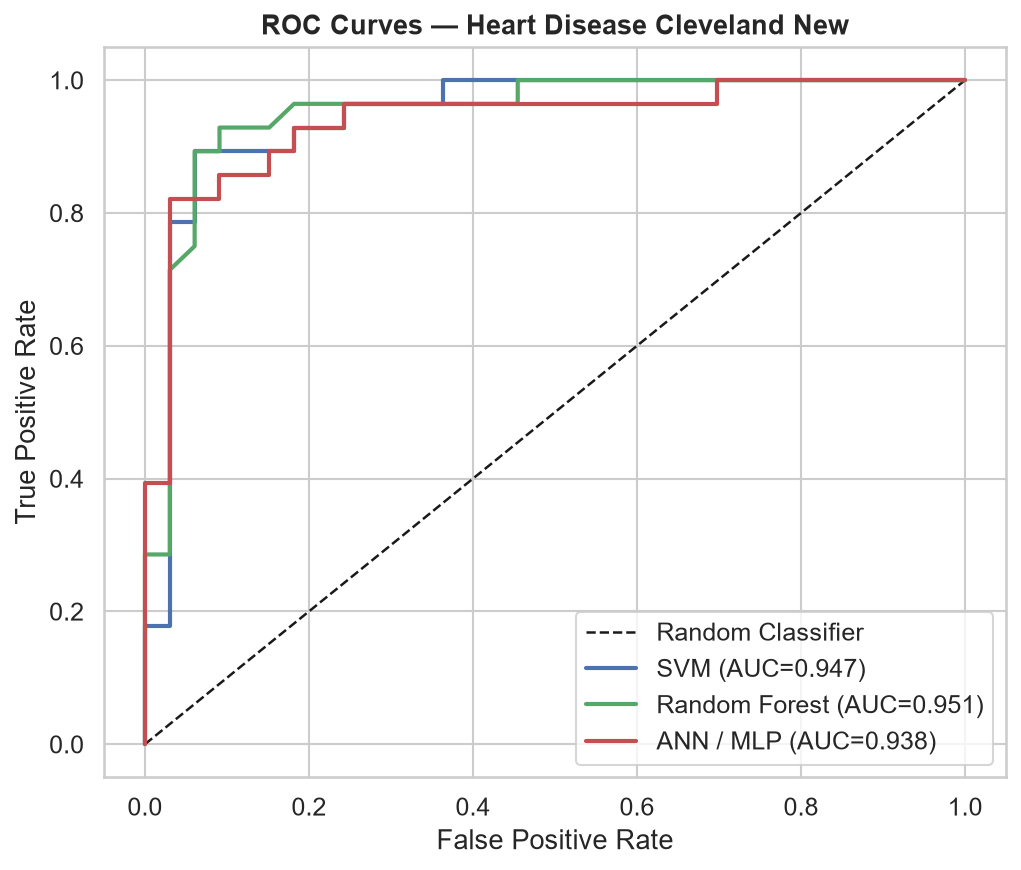
\includegraphics[width=0.85\columnwidth]{base_cle_roc.png}
\caption{ROC curves of the untuned baselines on the Cleveland hold-out set.}
\label{fig:baseroc}
\end{figure}

\subsection{Cooperative GA--PSO with SVM}
The ten-round run took 2346\,s. It selected 8 of the 13 attributes (age, sex, cp, fbs, thalach, exang, ca, thal) with $C=0.819$ and $\gamma=0.269$, for a fitness of 0.8068 (mean 10-fold F1 of 0.8468 before the penalty). The discarded attributes were trestbps, chol, restecg, oldpeak and slope. Removing the first three agrees with their weak individual correlation with the outcome ($|r|\le0.17$). Removing oldpeak ($r=0.43$) and slope ($r=0.34$) is less obvious, but both describe the exercise ST segment and overlap with exang, thalach and thal. Retaining fbs ($r=0.03$) is the least intuitive choice; we attribute it to the fact that a weak attribute changes the fold-averaged F1 by less than one patient, so the GA's choice among near-equal masks is partly arbitrary.

Table~\ref{tab:svm} lists the out-of-fold metrics, and Fig.~\ref{fig:cm} the confusion matrix. The model reaches an accuracy of 0.865 and an MCC of 0.727. Compared with the baseline, it is more precise on the disease class (0.877) but less sensitive (recall 0.820, 25 missed cases out of 139). This reflects the F1 objective and the smoother boundary implied by the lower $C$; a recall-weighted objective would suit screening better.

\begin{table}[t]
\caption{Cooperative GA--PSO SVM on Cleveland (10-fold out-of-fold)}
\label{tab:svm}
\centering
\begin{tabular}{@{}lc@{}}
\toprule
Metric & Value \\ \midrule
Accuracy & 0.865 \\
Macro precision / recall / F1 & 0.866 / 0.861 / 0.863 \\
Disease class precision / recall & 0.877 / 0.820 \\
No-disease class precision / recall & 0.855 / 0.902 \\
ROC AUC / average precision & 0.885 / 0.868 \\
MCC & 0.727 \\
TN, FP, FN, TP & 148, 16, 25, 114 \\
Features used & 8 of 13 \\ \bottomrule
\end{tabular}
\end{table}

\begin{figure}[t]
\centering
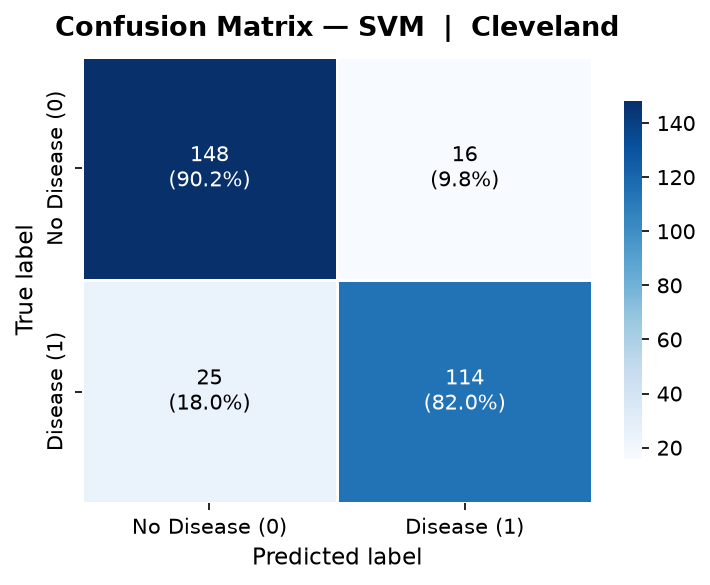
\includegraphics[width=0.65\columnwidth]{coop_svm_confusion_matrix.png}
\caption{Out-of-fold confusion matrix of the cooperative SVM.}
\label{fig:cm}
\end{figure}

\subsection{Behaviour of the cooperation}
Fig.~\ref{fig:conv} shows the best fitness after each round. In round 1 the GA reached 0.7877 under default SVM settings, and PSO raised this to 0.8068 by tuning $C$ and $\gamma$ on that mask. In rounds 2--10 neither the mask nor the hyperparameters changed. A repeated run reproduced every value exactly. For the SVM, therefore, the alternation reached a fixed point after one GA$\rightarrow$PSO pass: re-optimizing the mask under the tuned hyperparameters returned the same mask, and the warm-started, low-inertia swarm found nothing better near the previous optimum.

\begin{figure}[t]
\centering
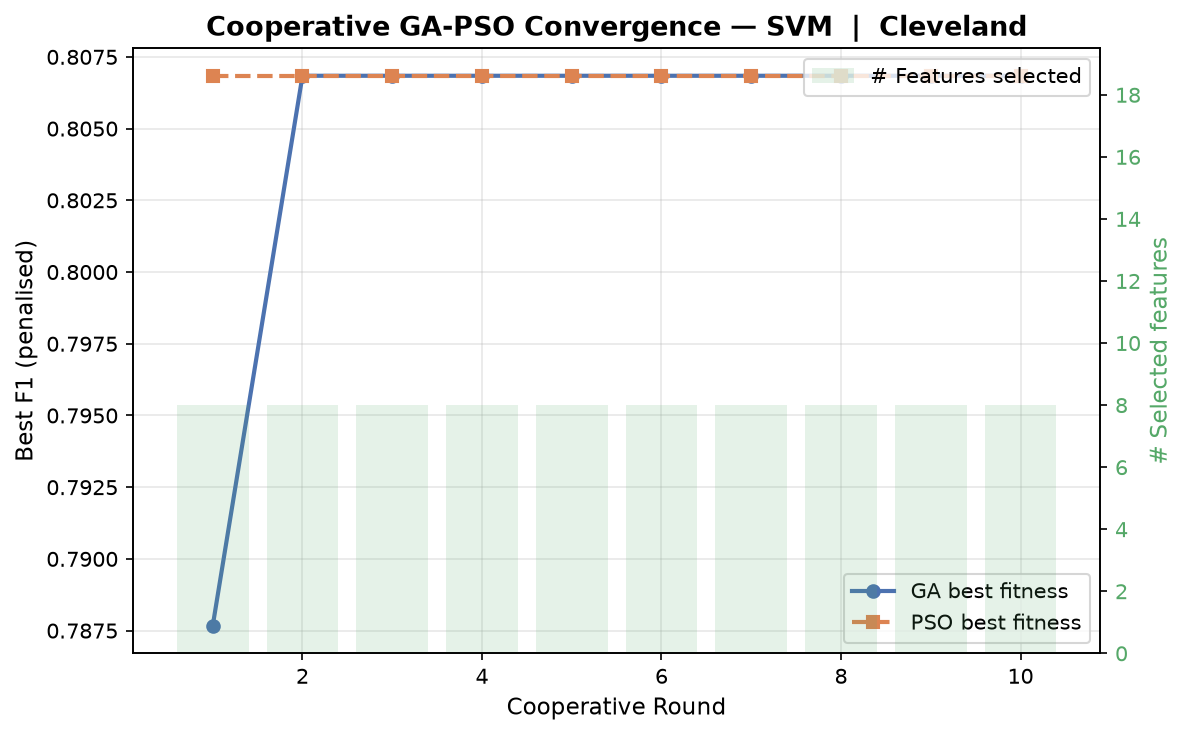
\includegraphics[width=0.9\columnwidth]{coop_svm_convergence.png}
\caption{Best GA and PSO fitness per round (SVM, Cleveland).}
\label{fig:conv}
\end{figure}

The random forest behaved differently (Table~\ref{tab:rf}). In round 2 the GA found a better 6-feature mask under the forest tuned in round 1, and PSO then improved on it again, which is the two-way benefit the design is meant to provide. The run plateaued at 0.8047 (raw F1 0.8347) and was stopped after six rounds because each PSO phase took 25--37 minutes. \todo{complete the RF run, report its selected features, and add the XGBoost run.}

\begin{table}[t]
\caption{Cooperative GA--PSO with RF on Cleveland (partial run)}
\label{tab:rf}
\centering
\begin{tabular}{@{}ccccc@{}}
\toprule
Round & GA fitness & PSO fitness & Trees / depth & Features \\ \midrule
1 & 0.7735 & 0.7766 & 190 / 7 & 6 \\
2 & 0.8005 & 0.8047 & 266 / 7 & 6 \\
3--6 & 0.8047 & 0.8047 & 266 / 7 & 6 \\ \bottomrule
\end{tabular}
\end{table}

\subsection{Overlap of the Statlog and Cleveland datasets}
\label{sec:overlap}
Comparing the two files record by record on all 13 attributes shows that every one of the 270 Statlog patients also appears in Cleveland, with the same label. Statlog is therefore a 270-patient subset of Cleveland, not a separate cohort. Results on Statlog say little about generalisation beyond Cleveland, and a model tuned on Cleveland and ``tested'' on Statlog would largely be scored on its own training patients. Studies that present the two as independent benchmarks should be read with this in mind.

%------------------------------------------------------------------------------
\section{Discussion}
\label{sec:disc}
The cooperative SVM's out-of-fold accuracy (0.865) is about four points above the untuned SVM's 5-fold accuracy (0.826). We do not claim this as an improvement yet, for two reasons. First, the protocols differ: 5-fold on 80\% of the data for the baseline, and 10-fold on all of it for the cooperative model. Second, the cooperative estimate is optimistic, because the folds that guided the search are also those used to evaluate it \cite{varma2006bias,cawley2010overfitting}. The lower AUC of the cooperative model (0.885, against 0.947 on the baseline hold-out set) also reflects the difference in protocol: pooling probabilities from ten separately fitted models can reduce AUC, while a single 61-patient split is highly variable.

The stalled SVM run suggests that cooperation pays off mainly when the best feature subset is sensitive to the hyperparameters. With an RBF SVM on 13 attributes and 8178 feasible masks, one pass was enough; with a random forest, the second round improved both the mask and the forest. Larger feature spaces, a less exploitative swarm (higher inertia or periodic re-randomisation), or noise-robust fitness estimates (repeated CV) may make further rounds productive. The cost is significant: for tree ensembles, evaluation should be parallelised or stopped early for poor particles.

\textbf{Limitations.} All results use one seed and one dataset; class balancing was not applied, although the positive rate of 45.9\% makes this less pressing; and the GA-only, PSO-only and sequential GA$\rightarrow$PSO comparison arms have not yet been run, so the specific contribution of the exchange is not yet isolated.

\todo{Before submission: (1) replace the out-of-fold evaluation with nested cross-validation, re-running the full search inside each outer fold; (2) evaluate baseline, GA-only, PSO-only, sequential and cooperative variants under the same outer folds over several seeds, with a paired statistical test \cite{demsar2006stats}; (3) add an independent dataset (e.g.\ Hungarian, Swiss or Z-Alizadeh Sani \cite{alizadehsani2013}). Update the abstract and conclusion with the new numbers.}

%------------------------------------------------------------------------------
\section{Conclusion}
We presented a cooperative GA--PSO scheme in which feature selection and hyperparameter tuning exchange solutions under one leakage-free objective. On the Cleveland data it produced an 8-attribute SVM with an out-of-fold accuracy of 0.865 and an MCC of 0.727. The round-by-round logs show that the exchange helped the random forest beyond its first round but reached a fixed point immediately for the SVM, which indicates where the method is worth its cost. We also showed that the Statlog heart dataset is contained in Cleveland, so it cannot confirm results obtained on Cleveland. Future work will use nested cross-validation, ablation against single-optimizer variants, an independent cohort, and SHAP-based explanation \cite{lundberg2017shap} of the selected models.

\bibliographystyle{IEEEtran}
\bibliography{refs}

\end{document}
